\chapter{Données et cadre expérimental}
\label{chapitre:donnees}

Ce chapitre décrit les données sur lesquelles le système est évalué, puis le cadre
expérimental correspondant. Il présente le corpus principal IceQube 2023, sa préparation et
ses variables dérivées, avant de détailler les campagnes injectées et la cohorte
IceTag-SLS.

% =====================================================================
\section{Corpus principal IceQube 2023}
% =====================================================================
\label{sec:donnees}

Le fichier \texttt{data/brut.csv} provient de la ferme du campus Macdonald de
l'Université McGill. Il contient 37\,839 mesures de 28 vaches entre le
1\textsuperscript{er} octobre et le 11 novembre 2023. Les variables sont agrégées à une
résolution nominale de 15 minutes. Le Tableau~\ref{tab:dataset} en décrit les
caractéristiques vérifiées.

\begin{table}[H]
  \centering
  \caption{Caractéristiques vérifiées du corpus IceQube 2023.}
  \label{tab:dataset}
  \small
  \begin{tabular}{lr}
    \toprule
    Caractéristique & Valeur \\
    \midrule
    Vaches & 28 \\
    Lignes & 37\,839 \\
    Résolution nominale & 15 minutes \\
    Période & 1 octobre--11 novembre 2023 \\
    Lignes par vache, médiane & 564 \\
    Lignes par vache, étendue & 244--2\,474 \\
    Doublons vache-temps & 0 \\
    \bottomrule
  \end{tabular}
\end{table}

\subsection{Variables brutes du corpus}
Les variables utilisées sont les pas, le \textit{Motion Index}, le temps couché, le temps
debout, les transitions et leur décomposition en levers et couchers
(Tableau~\ref{tab:variables_brutes}). Elles décrivent la quantité de mouvement et la
posture, contrairement à la mesure de l'asymétrie de démarche, de la douleur ou des lésions
du pied \citep{alsaaod2019automatic,oleary2020accelerometers}. Leur portée clinique est donc
indirecte.

\begin{table}[H]
  \centering
  \caption{Variables brutes du corpus IceQube 2023.}
  \label{tab:variables_brutes}
  \small
  \begin{tabular}{p{0.28\textwidth}p{0.60\textwidth}}
    \toprule
    Variable & Interprétation \\
    \midrule
    \textit{Steps} & Nombre de pas dans l'intervalle. \\
    \textit{Motion Index} & Intensité agrégée du mouvement mesuré par le capteur. \\
    \textit{Lying Time} & Temps couché dans l'intervalle. \\
    \textit{Standing Time} & Temps debout dans l'intervalle. \\
    \textit{Transitions} & Nombre total de transitions posturales. \\
    \textit{Transitions Up/Down} & Décomposition en levers et couchers. \\
    \bottomrule
  \end{tabular}
\end{table}

\subsection{Statistiques descriptives et variabilité inter-individuelle}
\label{subsec:statistiques_corpus}
Les distributions sont fortement asymétriques, comme le montre le
Tableau~\ref{tab:statistiques_brutes}~: la médiane des pas et des transitions par intervalle est nulle, tandis que les maxima sont
élevés. Cette structure écarte une normalisation gaussienne globale et motive des
comparaisons robustes propres à chaque vache et à chaque créneau horaire
\citep{leys2013detecting}.

\begin{table}[H]
  \centering
  \caption{Statistiques descriptives des variables de mouvement (par intervalle de 15~min).}
  \label{tab:statistiques_brutes}
  \small
  \begin{tabular}{lrrrr}
    \toprule
    Variable & Moyenne & Écart-type & Médiane & Maximum \\
    \midrule
    Pas & 4,0 & 15,4 & 0 & 387 \\
    \textit{Motion Index} & 25,5 & 103,7 & 5 & 3\,351 \\
    Transitions & 0,16 & 0,40 & 0 & 6 \\
    \bottomrule
  \end{tabular}
\end{table}

L'autocorrélation confirme que les intervalles successifs ne constituent pas des observations
indépendantes. Après mise sur une grille régulière et déduplication temporelle par vache, les
36\,879 mesures exploitables correspondent à environ 10\,000 observations indépendantes pour
le \textit{Motion Index}; au grain brut de 15 minutes, le temps d'autocorrélation intégré
est de l'ordre d'une heure pour les signaux d'activité. Au niveau de décision, les totaux
glissants de 12 heures portent ce temps à environ huit heures~: la médiane par vache tombe
alors à environ 17 points de décision indépendants. Les séries étant très inégales, cette
médiane ne se multiplie pas par l'effectif~; la somme des tailles effectives reste néanmoins de
l'ordre du millier sur l'ensemble du corpus, soit 1\,151 points pour les pas et 880 pour le
\textit{Motion Index}. Ce résultat justifie l'agrégation statistique par vache et le
rééchantillonnage groupé employés dans l'évaluation; il évite que la dépendance entre
intervalles produise des intervalles de confiance artificiellement étroits.

La variabilité entre vaches est considérable, comme le montre le
Tableau~\ref{tab:variabilite}. La moyenne de
pas par intervalle varie de 0,0 à 11,1 selon la vache, et le coefficient de variation
inter-vache atteint 0,50 pour les pas, 0,40 pour le \textit{Motion Index} et 0,41 pour les
transitions. Cette hétérogénéité interdit un seuil commun à tout le troupeau et justifie le
recours à une référence \emph{individuelle}, propre à chaque vache.

\begin{table}[H]
  \centering
  \caption{Variabilité inter-individuelle des principales variables (moyenne par vache).}
  \label{tab:variabilite}
  \small
  \begin{tabular}{lrrr}
    \toprule
    Variable & Moyenne/vache min & Moyenne/vache max & CV inter-vache \\
    \midrule
    Pas & 0,0 & 11,1 & 0,50 \\
    \textit{Motion Index} & 4,0 & 57,4 & 0,40 \\
    Transitions & 0,00 & 0,31 & 0,41 \\
    \bottomrule
  \end{tabular}
\end{table}

% =====================================================================
\section{Préparation des données et variables dérivées}
% =====================================================================
Cette section décrit les traitements appliqués aux mesures brutes avant la détection~: le
choix de la résolution, les contrôles d'admissibilité, la traçabilité des fichiers et la
construction des variables dérivées.

\subsection{Résolution temporelle}
\label{sec:resolution_temporelle}
L'agrégation à 15 minutes est conservée comme résolution nominale. Une résolution plus
fine multiplie le bruit et les intervalles vides sans ajouter d'information comportementale
exploitable à l'échelle d'un épisode de plusieurs heures~; une résolution plus grossière
masque les transitions posturales. Une résolution de 15 minutes permet d'avoir un compromis entre stabilité du
signal et granularité suffisante pour la persistance recherchée par les deux branches.

\subsection{Contrôles d'admissibilité}
Le chargement impose des dates interprétables, des identifiants non vides et des variables
numériques non négatives~; les durées posturales sont converties en minutes et la couverture
de chaque intervalle est conservée. Les données originales ne sont jamais modifiées par
l'évaluation~: chaque injection opère sur une copie en mémoire.

Le corpus regroupe 16 vaches suivies pendant moins de 14 jours et 12 vaches disposant de
séries plus longues. Pour être admissible à l'évaluation synthétique, une vache doit disposer
d'au moins 14 jours de mesures, d'une période future après la période de référence et de
valeurs informatives pour les pas, le \textit{Motion Index} et les transitions. Ces critères
retiennent 11 vaches. Les 28 vaches demeurent néanmoins disponibles dans l'interface~; la
restriction à 11 animaux s'applique uniquement au protocole expérimental.

La Figure~\ref{fig:admissibilite} présente les identifiants des vaches sur l'axe vertical et la
durée des séries sur l'axe horizontal. Les 11 vaches admissibles sont représentées en vert et
les 17 vaches non admissibles en gris. Le trait pointillé représente le seuil de 14 jours.
Parmi les vaches non admissibles, 16 se trouvent sous ce seuil. La vache 8144 le dépasse,
mais ses signaux ne sont pas informatifs dans la période future, ce qui explique son exclusion.

\begin{figure}[H]
  \centering
  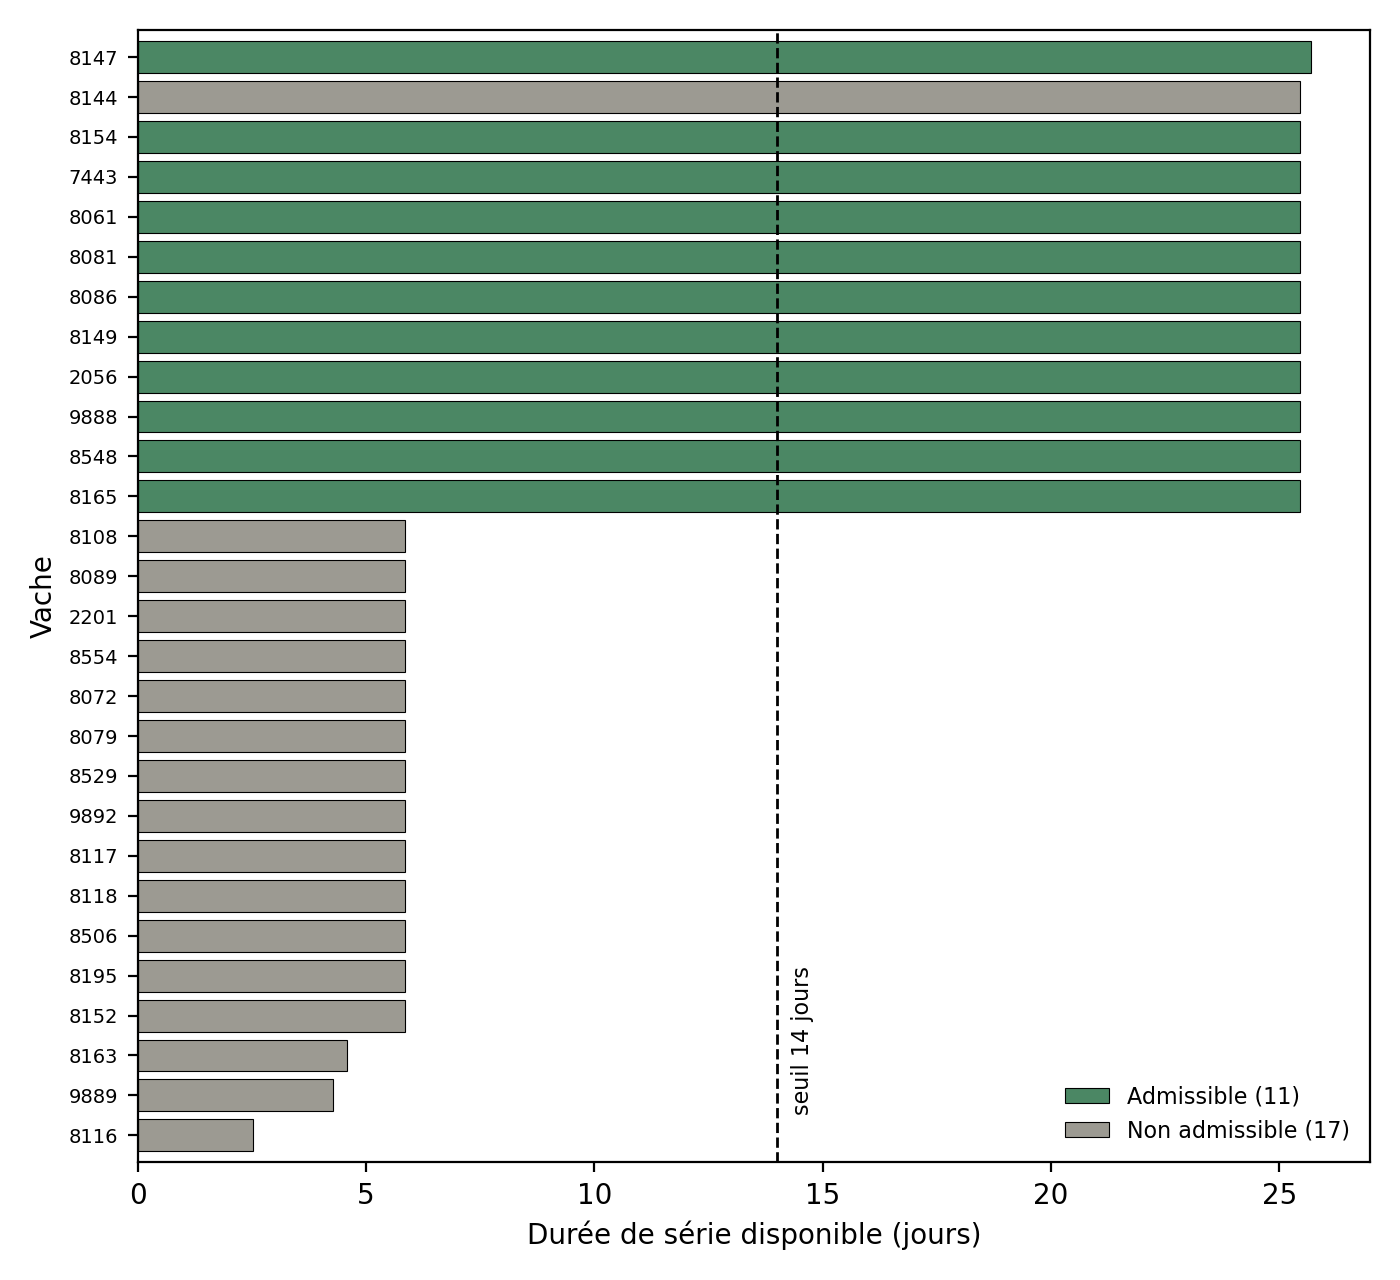
\includegraphics[width=0.80\textwidth]{figures/cow_admissibility.png}
  \caption{Admissibilité des vaches.}
  \label{fig:admissibilite}
\end{figure}

\subsection{Traçabilité et provenance des données}
La provenance du corpus a été vérifiée en confrontant ses valeurs à celles du système
commercial CowAlert (IceRobotics), qui restitue les mêmes mesures IceQube
\citep{icerobotics2012cowalert}. Pour les 5 vaches dont les mesures ont pu être relevées
depuis ce système, les deux sources de données, soit le corpus brut et l'export CowAlert,
sont alignées sur la clé vache-début d'intervalle, après vérification de l'absence de
doublons. Les 7\,631 intervalles communs représentent 97,5\,\% des 7\,823 lignes de
l'export CowAlert. Pour ces intervalles, les pas, le \textit{Motion Index} et les
transitions sont identiques, avec une corrélation parfaite de 1,0. Le corpus correspond
donc aux mesures restituées par le système officiel pour ces vaches. À noter que cette
vérification porte sur 5 des 28 vaches. Seules les corrélations agrégées sont rapportées,
puisque l'export CowAlert est confidentiel.

\subsection{Variables dérivées}
La chaîne de traitement calcule plusieurs variables dérivées à partir de chaque variable
brute, comme le montre le Tableau~\ref{tab:features}. Elle produit des agrégats par intervalle,
des transformations logarithmiques qui atténuent l'asymétrie, des z-scores robustes globaux
et glissants, ainsi qu'un indicateur de couverture. Ces variables alimentent IF, LOF et les
règles de cohérence qui leur sont associées. HYPO et INSTABILITÉ utilisent plutôt des ratios
calculés par rapport à la référence individuelle.

\begin{table}[H]
  \centering
  \caption{Familles de variables dérivées par variable comportementale brute.}
  \label{tab:features}
  \small
  \begin{tabular}{p{0.32\textwidth}p{0.56\textwidth}}
    \toprule
    Famille & Description \\
    \midrule
    Agrégats & Somme et moyenne par intervalle de 15 minutes. \\
    Transformations log & $\log(1+x)$ sur la somme et la moyenne. \\
    Z-score robuste global & Centrage par la médiane, échelle par l'écart absolu médian (MAD). \\
    Z-score robuste glissant & Même principe sur une fenêtre mobile de 24~intervalles. \\
    Couverture & Rapport entre échantillons observés et attendus par intervalle. \\
    \bottomrule
  \end{tabular}
\end{table}

% =====================================================================
\section{Cadre expérimental}
\label{sec:cadre_experimental}
% =====================================================================
Le cadre expérimental comprend deux campagnes injectées principales, une campagne de stress
complémentaire et une cohorte observationnelle distincte. La
Figure~\ref{fig:plan_etude} présente cette organisation.

\begin{figure}[H]
  \centering
  \begin{tikzpicture}[
    box/.style={rectangle, draw=black!55, rounded corners=2pt, align=center,
      minimum height=2.1cm, minimum width=3.7cm, text width=3.4cm, inner sep=6pt, font=\small},
    arrow/.style={-{Stealth[length=2.2mm]}, thick, black!65}]
    \node[box, fill=ifblue!10] (main) {IceQube 2023\\28 vaches};
    \node[box, fill=rulegreen!10, right=0.4cm of main] (split) {Référence 60\,\%\\futur 40\,\%};
    \node[box, fill=loforange!10, right=0.4cm of split] (inject) {HYPO: 44\\INSTABILITÉ: 132\\stress: 198};
    \node[box, fill=profgray!10, right=0.4cm of inject] (eval) {Comparaison propre-injectée\\unité: vache};
    \draw[arrow] (main) -- (split); \draw[arrow] (split) -- (inject); \draw[arrow] (inject) -- (eval);
    \node[box, fill=ifblue!7, below=0.8cm of main] (sls) {IceTag-SLS 2019\\14 vaches};
    \node[box, fill=rulegreen!7, below=0.8cm of split] (pre) {Sept jours\\avant le SLS};
    \node[box, fill=profgray!7, below=0.8cm of inject] (conc) {Concordance exploratoire\\sans réglage};
    \draw[arrow] (sls) -- (pre); \draw[arrow] (pre) -- (conc);
  \end{tikzpicture}
  \caption{Plan d'étude.}
  \label{fig:plan_etude}
\end{figure}

Les trois niveaux présentés sont les suivants~:
\begin{itemize}
  \item le premier niveau évalue HYPO sur 44 événements et le compare aux trois variantes
  fondées sur IF ou LOF ainsi qu'au comparateur pédométrique;
  \item le deuxième niveau applique 132 scénarios afin d'explorer INSTABILITÉ et cinq règles
  de fusion;
  \item le troisième niveau analyse une cohorte IceTag-SLS de l'hiver 2019 composée de
  14 vaches. Il utilise les mesures des sept jours précédant le score locomoteur et ne sert
  pas à régler le système.
\end{itemize}

Dans chacun des deux premiers niveaux, un scénario est injecté dans une copie distincte de la
période future, puis comparé à l'exécution propre de la même vache. Ce plan forme un banc
d'essai contrefactuel reproductible~: l'événement synthétique est le seul changement
volontaire entre l'exécution propre et l'exécution injectée, ce qui permet de mesurer la
réponse du détecteur sans modifier la période de référence ni optimiser les seuils sur les
sorties observées.

Une campagne de stress complémentaire réexécute aussi HYPO et les quatre comparateurs sur
six formes moins favorables, à trois positions par vache. Elle est séparée des résultats qui
ont servi à construire le système. Son protocole JSON interdit tout nouveau réglage et
apparie l'aire de l'enveloppe numérique~: pour chaque famille modifiée, l'aire discrète sous
l'enveloppe, calculée sur les intervalles effectivement conservés, est égale à celle du
profil modéré graduel de 48 heures. Cette contrainte évite d'attribuer à la forme temporelle
un effet qui proviendrait seulement d'une enveloppe programmée plus intense; elle ne garantit
pas une amplitude physiologique ou comportementale identique. Le contrôle négatif modifie
uniquement les pas avec la même aire numérique; le scénario de données manquantes retire un
bloc contigu de 12 heures après cet appariement.

\subsection{Campagne principale et ablation du module HYPO}
La campagne principale construit quatre événements pour chacune des 11 vaches admissibles,
soit 44 événements~:
\begin{itemize}
  \item le profil \textbf{léger} diminue progressivement les pas, le mouvement et les
  transitions, puis transfère une part du temps debout vers le temps couché pendant 36 heures;
  \item le profil \textbf{modéré} applique la même évolution pendant 48 heures;
  \item le profil \textbf{marqué} l'applique pendant 60 heures;
  \item le contrôle bref dure trois heures et ne devrait pas former un épisode persistant.
\end{itemize}
Cette campagne reprend le cadre contrefactuel de la Section~\ref{sec:cadre_experimental}.
Pour HYPO, l'exécution propre de la même vache est soustraite lors du calcul des métriques
attribuables.

L'étude d'ablation évalue l'apport de la structure temporelle et multivariée de HYPO en la
comparant à quatre configurations simplifiées ou alternatives. Les cinq variantes sont
appliquées aux mêmes fenêtres~:
\begin{itemize}
  \item (A) HYPO temporel multivarié;
  \item (B) IF suivi des règles de persistance;
  \item (C) IF ponctuel;
  \item (D) LOF suivi des règles;
  \item (E) un comparateur pédométrique restreint au seul canal des pas.
\end{itemize}
Les comparaisons appariées sont calculées après agrégation par vache. Une analyse OFAT
conserve les mêmes 11 vaches, les mêmes fenêtres et la même graine, puis modifie séparément
dix paramètres autour de la référence. Elle évalue une robustesse locale et ne sélectionne
pas une nouvelle configuration.

\subsection{Extension bidirectionnelle et contrôles de confusion}
Douze scénarios sont appliqués à chacune des onze vaches admissibles, soit 132 événements,
selon le même cadre contrefactuel. L'enveloppe est progressive, avec montée, plateau et
retour, et la somme des temps couché et debout est conservée. Le
Tableau~\ref{tab:profils_detection} décrit ces douze scénarios.

\begin{table}[H]
  \centering
  \caption{Scénarios de l'évaluation technique.}
  \label{tab:profils_detection}
  \small
  \begin{tabular}{p{0.27\textwidth}p{0.18\textwidth}p{0.43\textwidth}}
    \toprule
    Famille & Nombre & Rôle \\
    \midrule
    Hypoactivité légère, modérée, marquée & 33 & Baisse progressive de plusieurs signaux sur 24 à 48 h. \\
    Instabilité légère, modérée, marquée & 33 & Mouvement relatif, transitions et posture sur 8 à 16 h. \\
    Instabilité puis hypoactivité & 11 & Séquence séparée par 24 h. \\
    Pic capteur, exercice bref, manipulation & 33 & Contrôles brefs qui doivent être rejetés. \\
    Activité de type œstrus & 11 & Confondant d'hyperactivité coordonnée. \\
    Hypoactivité non locomotrice & 11 & Confondant causal indiscernable avec les capteurs seuls. \\
    \bottomrule
  \end{tabular}
\end{table}

L'amplitude modérée des pas atteint 29\,\%, valeur ancrée sur un ordre de grandeur publié
autour d'un parage thérapeutique \citep{paudyal2021lying}. Les amplitudes des autres signaux
sont des hypothèses de test et non des estimations cliniques.

\subsection{Cohorte IceTag-SLS de l'hiver 2019}
\label{subsec:corpus_mcgill}

Le développement et l'évaluation technique du système ont d'abord été réalisés sur le corpus
IceQube 2023. La cohorte IceTag-SLS 2019, devenue accessible dans un second temps, a ensuite
été exploitée sans modifier la configuration ni les seuils du détecteur.

Les deux ensembles de données ne sont ni fusionnés ni appariés animal par animal. Le corpus
IceQube 2023 sert à l'évaluation technique du système, tandis que la cohorte IceTag-SLS 2019
fournit une confrontation observationnelle distincte avec des scores locomoteurs contemporains.
Cette cohorte provient du même campus, mais d'une période et d'un dispositif différents.
Le SLS représente la somme de quatre composantes binaires et varie de 0 à 4. L'analyse retient le
score du 12 mars 2019 et les données capteurs strictement antérieures. Une vache doit avoir
une période de référence suffisante et au moins 70\,\% de couverture dans les sept jours précédents.
Quatorze vaches sont évaluables: deux ont un SLS de 0, neuf un SLS de 1 et trois un SLS de 2.
Aucun SLS de 3 ou 4 n'est observé. Le seuil SLS~$\geq2$ constitue une séparation
exploratoire, non un diagnostic imposé par le protocole source.

\subsection{Protocole de l'analyse SLS}
La configuration hiérarchique est appliquée sans utiliser les scores pour entraîner le
détecteur ou régler ses seuils. Dans l'analyse finale, cette fusion et le nombre de notifications
dans les sept jours précédant le 12 mars 2019 sont retenus comme analyse principale. Sont également
rapportées la fraction du temps en épisode, la surveillance d'instabilité et le score
maximum. Les comparaisons utilisent l'AUC descriptive, le test de Mann-Whitney et la
corrélation de Spearman au niveau de la vache. Avec seulement trois SLS~$\geq2$, ces mesures
restent exploratoires. Pour tenir compte exactement du petit effectif et des ex æquo, toutes
les répartitions possibles des trois étiquettes positives parmi les quatorze vaches sont
énumérées pour l'AUC. L'analyse est ensuite répétée dans le seul groupe
\textit{Exercise}; le groupe sans exercice ne contient aucun SLS~$\geq2$ et son AUC n'est
donc pas estimable. Un test exact de Fisher quantifie l'association entre traitement et
classe SLS, et une analyse leave-one-positive-out vérifie l'influence de chacune des trois
vaches positives. Enfin, une analyse de sensibilité ajoutée après l'analyse principale emploie
un test exact max-stat pour contrôler la recherche parmi les cinq variantes de fusion pour le
nombre de notifications, puis parmi les vingt combinaisons formées par les cinq variantes et
les quatre métriques. Son caractère postérieur impose une portée exploratoire; la valeur $p$
globale non ajustée est conservée comme résultat descriptif.
